%% Lee
%% In dissertation, change 
%    section* to chapter 
%    subsection* to section
%    subsubsection* to subsection


% #######################################################################################################################################
\chapter{Detailed System Description}
\label{sec:Detailed System Description}

A detailed flow diagram and block diagram of the sub-system column can be seen in figures \ref{fig:DetailedFlowDiagram} and \ref{fig:DetailedBlockDiagram} respectively.
\begin{figure}[h]
% the [] contains position info e.g. [!t] means here
\centering
\captionsetup{justification=centering}
\captionsetup{width=.9\linewidth}
\centerline{
\mbox{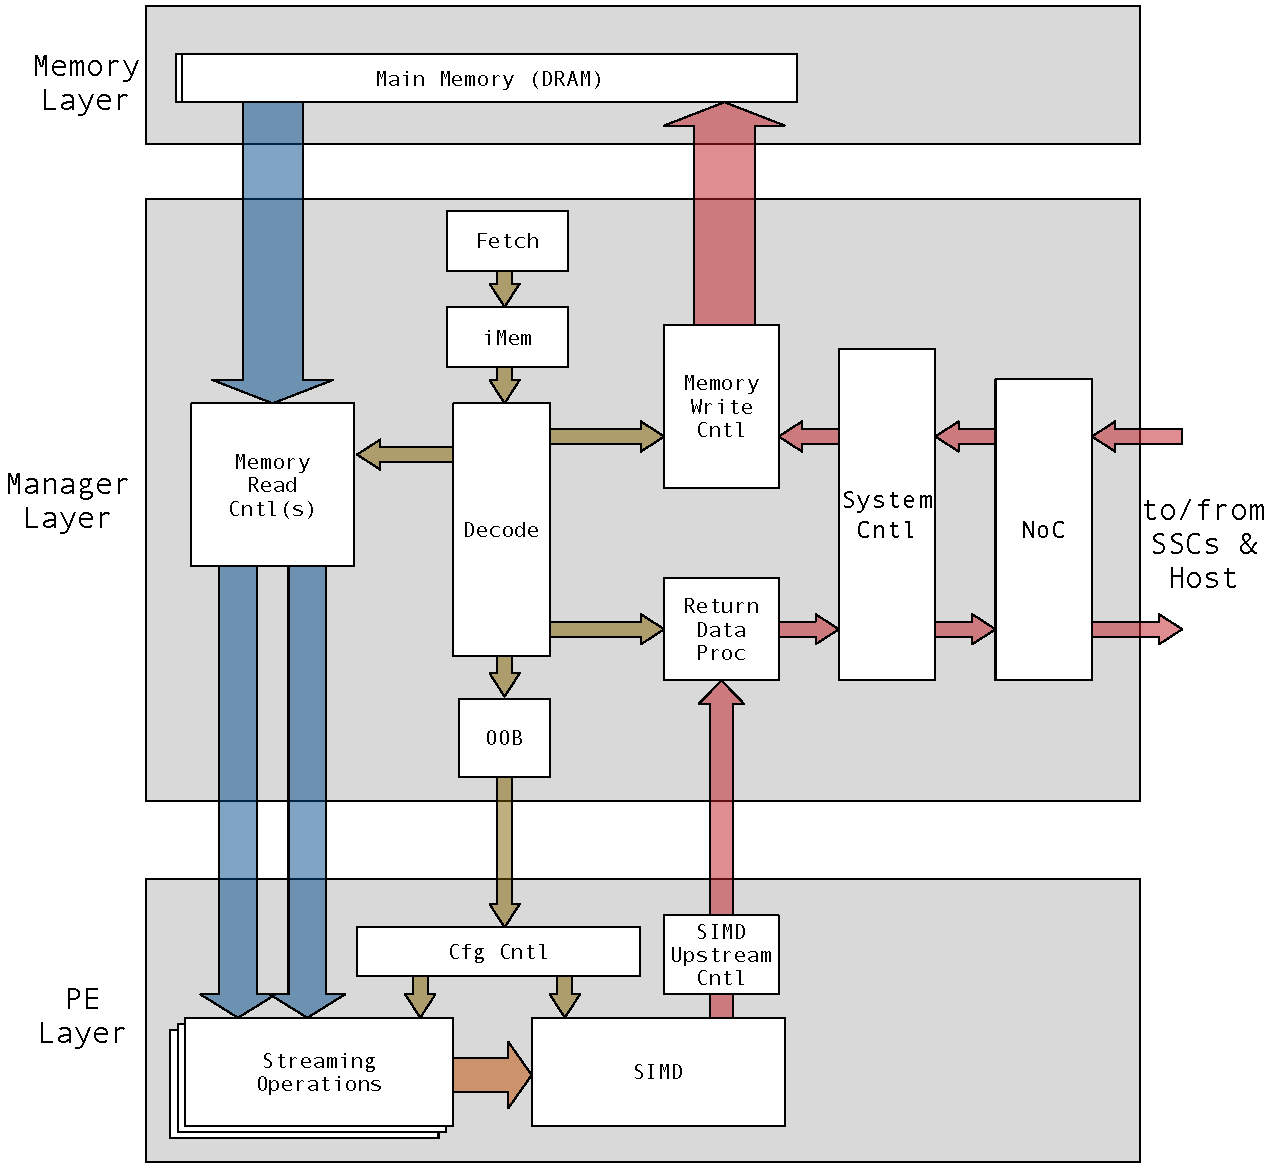
\includegraphics[scale=0.5]{DetailedFlowDiagram}}
}
\center\caption{Sub-System Column (SSC) Flow Diagram}
\label{fig:DetailedFlowDiagram}
\end{figure}

\section{Manager}
\label{sec:manager}

A block diagram of the manager can be seen in figure \ref{fig:Manager block diagram}.
\begin{figure}[h]
\centering
\captionsetup{justification=centering}
\captionsetup{width=.9\linewidth}
\centerline{
\mbox{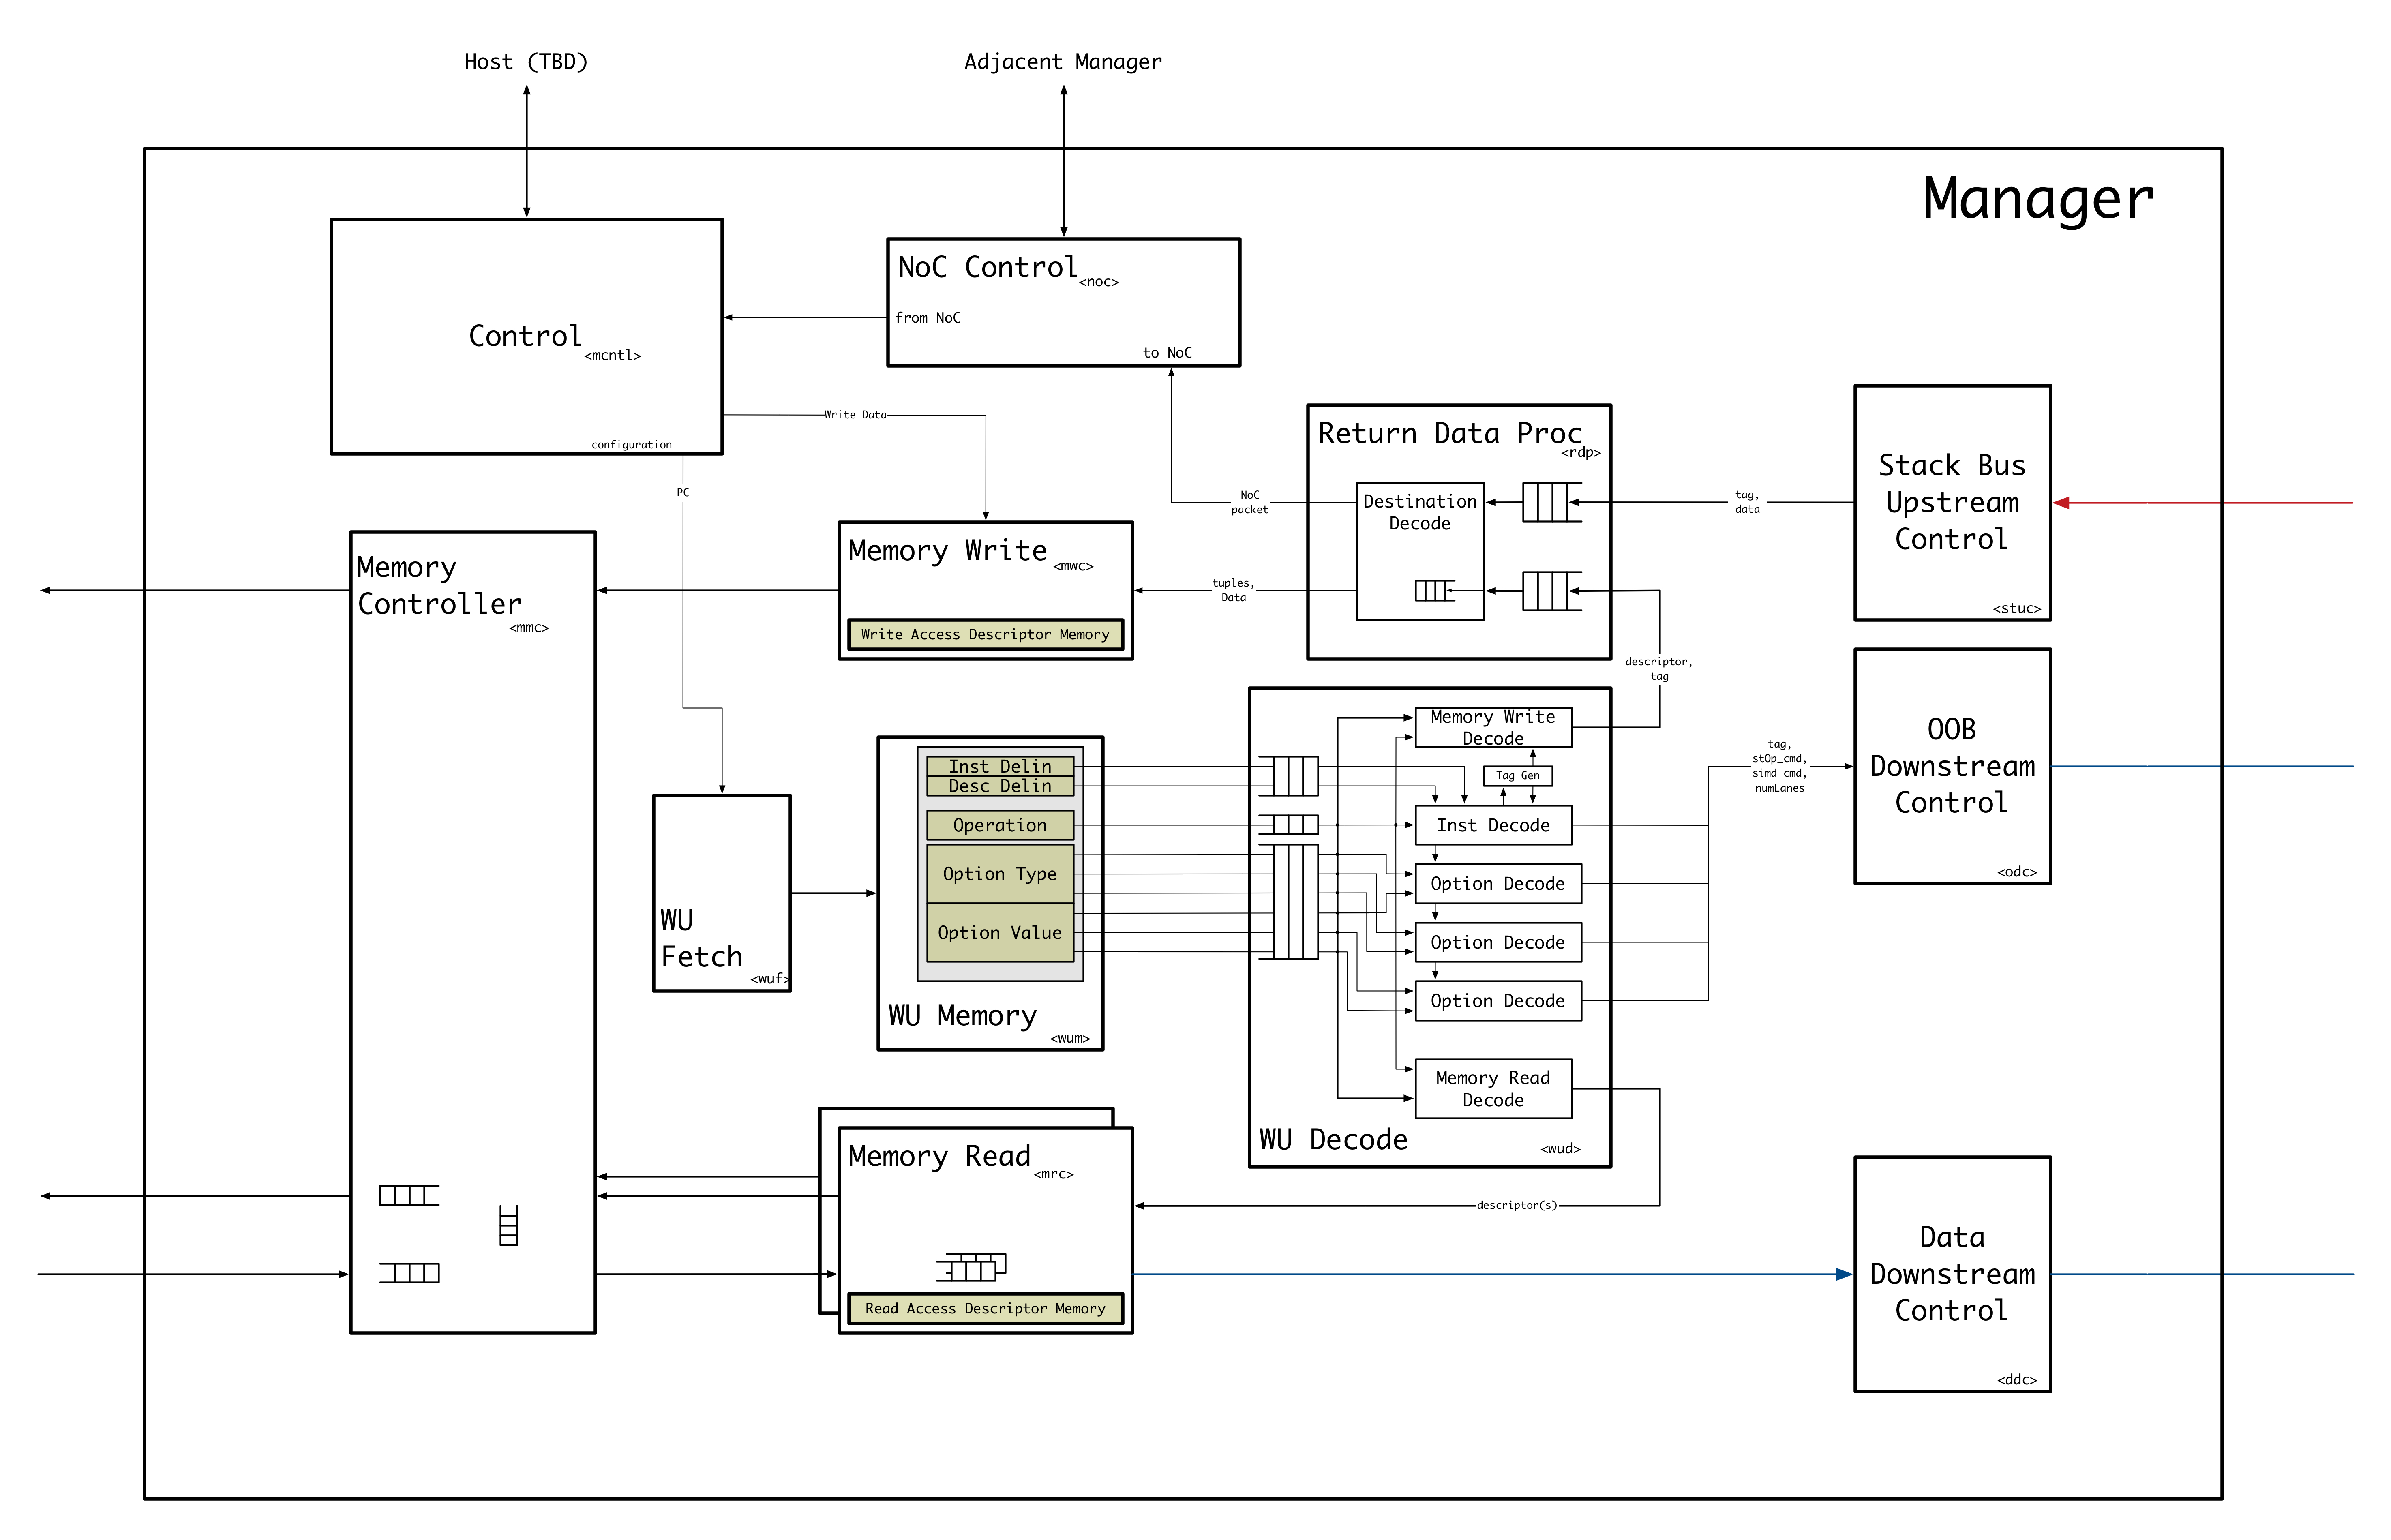
\includegraphics[width=1\linewidth]{Manager}}
}
\center\caption{Manager block diagram}
\label{fig:Manager block diagram}
\end{figure}

\subsection{System controller}
\label{sec:System controller}

The system controller is responsible for initialization and general system configuration.
A block diagram can be seen in figure \ref{fig:System controller}.

\begin{figure}[h]
% the [] contains position info e.g. [!t] means here
\centering
\captionsetup{justification=centering}
\captionsetup{width=.9\linewidth}
\centerline{
\mbox{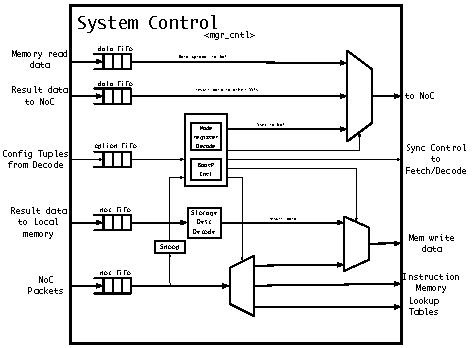
\includegraphics[scale=1.5]{systemControllerBlockDiagram}}
}
\center\caption{System controller}
\label{fig:System controller}
\end{figure}

\subsubsection{Initial Boot}
\label{sec:Initial Boot}

The system controller is responsible for performing the initial \ac{bootp} process.
This involves quiescing the system after reset and downloading the initial boot instructions from the host.

After reset, the controller keeps the instruction fetch logic disabled and expects unsolicited \ac{noc} packets from the host which contain the initial boot code.
The host will unsolicitedly send the \ac{bootp} code over the \ac{noc} to each \ac{ssc}.
The controller in each \ac{ssc} decodes the \ac{noc} packets and writes the data directly into instruction memory.
Currently each \ac{noc} \ac{mtu} packet contains 16 instruction memory entries (see figure \ref{fig:Host boot code packet}).
The number of initial instruction entries is hard-coded but it is anticipated a standard on-chip protocol such as \ac{jtag} will be used to set initial \ac{bootp} configuration.
Once the host has sent the \ac{bootp} code, each \ac{ssc} controller releases its instruction fetch block.

It is anticipated that the initial \ac{bootp} code will not contain operational instructions but only configuration instructions to download configuration tables, the \ac{pe} \ac{simd} instruction memory and the \ac{ann} parameters.
For example, to download the \ac{ann} parameters, the \ac{bootp} instructions will include a configuration sync and a configuration data download.

The first \ac{bootp} instruction will be a configuration sync sent to the host to indicate the initial \ac{bootp} is complete and \ac{ann} parameters are ready to be received.
After the configuration sync is sent to the host, the configuration data instruction will prepare the \ac{ssc} to receive data from the host and the host will then start sending configuration data. 
The size of the data is known by both the \ac{ssc} via the instruction and the host.
The \ac{ann} parameters can be downloaded using multiple downloads.
Once \ac{ann} parameters and system tables are downloaded, the last instruction can be another configuration data instruction download to load operational code.

\begin{figure}[h]
  \vspace{5mm}
  \begin{minipage}{1\textwidth}
  %\begin{subfigure}{1\textwidth}
    \centering
    \captionsetup{justification=centering, skip=10pt}
    \begin{bytefield}[bitwidth=0.49em, endianness=big]{77}
      \bitheader{0,8,16,24,32,40,48,56,64,68,74,76} \\
      \begin{rightwordgroup}{\scriptsize Unicast Bitfield header}
        \bitbox{2}{\rotatebox{90}{\tiny SOM}} & \bitbox{7}{\scriptsize src} & \bitbox{2}{\tiny M} & \bitbox{1}{\rotatebox{90}{\tiny prio}} & \bitbox{64}{\tiny destination SSC bitfield} 
      \end{rightwordgroup}  \\
      \begin{rightwordgroup}{\scriptsize Data Cycle}
        \bitbox{2}{\rotatebox{90}{\tiny MOM}} & \bitbox{1}{} & \bitbox{4}{\tiny type} & \bitbox{3}{\tiny pyld\\ \vspace{-0em} type} & \bitbox{1}{} & \bitbox{1}{\tiny P\\ V} & \bitbox{7}{\tiny NA} & \bitbox{57}{\tiny Instruction memory entry}
      \end{rightwordgroup}  \\
      \bitbox[]{76}{$\vdots$} \\[1ex]
      \begin{rightwordgroup}{\scriptsize Data Cycle}
        \bitbox{2}{\rotatebox{90}{\tiny EOM}} & \bitbox{1}{} & \bitbox{4}{\tiny type} & \bitbox{3}{\tiny pyld\\ \vspace{-0em} type} & \bitbox{1}{} & \bitbox{1}{\tiny P\\ V} & \bitbox{7}{\tiny NA} & \bitbox{57}{\tiny Instruction memory entry}
      \end{rightwordgroup}  \\
    \end{bytefield}
    \captionsetup{justification=centering, skip=9pt}
    \vspace{-0.5cm}
    \captionof{figure}{Host boot code download \ac{noc} packet}
    \label{fig:Host boot code packet}
  \end{minipage}
\end{figure}

\subsection{Instruction Decoder}
\label{sec:Instruction Decoder}

In figure \ref{fig:Manager block diagram}, instructions are read from WU memory by the WU fetch block and the output of the memory is passed to the WU decoder block.

\subsubsection{Compute Instructions}
\label{sec:Decoding Compute Instructions}

The operation descriptor is decoded and a \ac{stop} pointer and a \ac{simd} \ac{pc} pointer are extracted. 
A sequential tag is generated and along with the \ac{stop} and \ac{simd} pointers and immediately sent to the \ac{pe} inside an \ac{oob} control packet.
The \ac{stop} pointer specifies what streaming operation is to take place on the data directly streamed to the \ac{pe}. 
The SIMD pointer is essentially a \ac{pc} counter that the \ac{simd} will jump to to process the result from the \ac{stop}.
The \ac{pe} will immediately start preparing for downstream oeprand data.
If the \ac{simd} operation ncludes result data being returned to the manager, the tag will be included in the upstream result data packet.

The memory read descriptors are decoded to identify the target memory read controller and the storage descriptor pointer directed to the appropriate memory read block.
There is a memory read block associated with each of the operand streams and are responsible for generating memory requests and directing the \ac{dram} data to all the execution lane streams.
A request block inside the memory read block immediately start pre-fetching the memory data by sending memory requests to the \ac{dram}.
A stream block inside the memory read block immediately starts waiting for data from the \ac{dram} and will direct \ac{dram} data to the appropriate execution lane.

The memory write descriptor is decoded and the storage descriptor pointer extracted and along with the tag are sent to the return data processor. The tag is sent to match with the returned data.
Currently the system only allows in-order data but the tag is provided for extensibility.

At this point all the blocks that take part in a compute operation on a group of \acp{an} are perforiming the various tasks.
As mentioned in section \ref{sec:Common Bus Signalling}, the inputs to many blocks employ \acp{fifo}. 
This allows blocks to pipeline tasks to absorb any latencies, they also allow blocks to start sending data to a destination block before that block has been configured to receive the data.
The \ac{fifo} will assert a flow control signal until the block is ready to receive.
In practice, the instruction decode logic batch decodes up to eight instructions and sends descriptor contents to dependent blocks where they are also pipelined.

\subsubsection{Configuration Instructions}
\label{sec:Decoding Configuration Instructions}

The configuration instructions are responsible for :
\begin{outline}
 \1 performing synchronization between the \ac{ssc} and other \acp{ssc} or the host system.
 \1 performing data download and upload operations
\end{outline}

The configuration packets are broken into two types, configuration data and configuration sync.
\iffalse
Currently the sync instruction has been implemented.
It is assumed at this point that adequate infrastructure and extensibility has been built into the system to allow implementation without adding significant amouts of logic.
\fi

The configuration instruction contains a single descriptor with one, two or three option tuples.

The sync instruction descriptor contains a single configuration sync option tuple. The 24-bit option value contains a 3-bit mode register identifier and a 21-bit mode register.
There are currently four mode registers defined, "Send", "Wait", "Pause" and "Flush". Each register has fields specific to the mode as seen in figure \ref{fig:Sync instruction}.

The data configuration instruction descriptor contains a configuration data option tuple and a storage descriptor tuple and optionally a target tuple. 
The configuration data option value is 24-bits with a 3-bit mode register identifier and a 21-bit mode register.
There are currently four mode registers defined, "instruction download", "sync group download", "memory download" and "memory upload". Each register has fields specific to the mode as seen in figure \ref{fig:Data transfer instruction}.

\paragraph{Sync Send}

The register fields can be seen in register \ref{reg:Sync Send mode register}.
The decoder sends the sync option tuple to the system controller.
A sync \ac{noc} packet is constructed based on the register contents sent over the \ac{noc}.
If the group pointer enable bit is set, the system conntroller uses the pointer to index into a 64 table. 
Each table entry is a 64-bit bitfield indicating which \acp{ssc} are a part of the group.
If the all flag is set, the sync packet will be sent to all \acp{ssc}.
if the host flag is also set, the host bit in the \ac{noc} packet will be set.
\begin{register}{H}{Sync Send mode register}{}%{0x250} name=example
  \label{reg:Sync Send mode register}
  % sizes 
  %\tiny 	
  %\scriptsize 	
  %\footnotesize
  %\small 	
  %\normalsize 	
  %\large 	
  %\Large 	
  %\LARGE 	
  \vspace{-20pt}
  \regfield{{\scriptsize Mode Reg ID         }}{ 3}{21}{000}%
  \regfield{{\scriptsize Not used            }}{12}{ 9}{{NA}}%
  \regfield{{\scriptsize Group Pointer enable}}{ 1}{ 8}{{en}}%
  \regfield{{\scriptsize Sync Group pointer  }}{ 6}{ 2}{{gPtr}}%
  \regfield{{\scriptsize Send to all SSCs    }}{ 1}{ 1}{{{\tiny all}}}%
  \regfield{{\scriptsize Send to host        }}{ 1}{ 0}{{{\tiny  host}}}%
  %\center\caption{Sub-System Column (SSC) Block Diagram}
  %\reglabel{Reset}\regnewline%
\end{register}

\paragraph{Sync Wait}

The register fields can be seen in register \ref{reg:Sync Send mode register}.
The decoder sends the sync option tuple to the system conntroller.
The instruction decoder will stop processing any more instructions until the release signal is asserted from the system conntroller.
The wait option informs the system conntroller to start expecting sync send packets from other \acp{ssc} and/or the host.
Based on the register values, the system conntroller will assert the release signal to the instruction decoder only once sync send packets have been received from all specified sources.
If the group pointer enable bit is set, the system conntroller uses the pointer to index into a 64 table. 
Each table entry is a 64-bit bitfield indicating from which \acp{ssc} a sync send packet should be received.
If the all flag is set, all sync send packets are expected from all \acp{ssc}.
if the host flag is also set, a sync send packet is expected from the host.
\begin{register}{H}{Sync Wait mode register}{}%{0x250} name=example
  \label{reg:Sync Wait mode register}
  \vspace{-20pt}
  \regfield{{\scriptsize Mode Reg ID         }}{ 3}{21}{001}%
  \regfield{{\scriptsize Not used            }}{12}{ 9}{{NA}}%
  \regfield{{\scriptsize Group Pointer enable}}{ 1}{ 8}{{en}}%
  \regfield{{\scriptsize Sync Group pointer  }}{ 6}{ 2}{{gPtr}}%
  \regfield{{\scriptsize Receive from all SSCs    }}{ 1}{ 1}{{{\tiny all}}}%
  \regfield{{\scriptsize Receive from host        }}{ 1}{ 0}{{{\tiny  host}}}%
  %\center\caption{Sub-System Column (SSC) Block Diagram}
  %\reglabel{Reset}\regnewline%
\end{register}


\paragraph{Sync Pause}

The register fields can be seen in register \ref{reg:Sync Pause mode register}.
The decoder sends the sync option tuple to the system conntroller and ceases decoding instructions.
If the indefinitely flag is set, instruction decode will not restart until the release signal is asserted from the system conntroller, otherwise the decoder will wait a number of clock cycles specified by the count field and then restart decoding instructions.
\begin{register}{H}{Sync Pause mode register}{}%{0x250} name=example
  \label{reg:Sync Pause mode register}
  \vspace{-10pt}
  \regfield{{\scriptsize Mode Reg ID         }}{ 3}{21}{010}%
  \regfield{{\scriptsize Wait <count> cycles }}{12}{ 9}{{count}}%
  \regfield{{\scriptsize Not used            }}{ 8}{ 1}{{NA}}%
  \regfield{{\scriptsize Indefinitely        }}{ 1}{ 8}{{Ind}}%
  %\center\caption{Sub-System Column (SSC) Block Diagram}
  %\reglabel{Reset}\regnewline%
\end{register}

\paragraph{Sync Flush}

There are currently no fields implemented in the sync flush register.
This instruction is designed to pause instruction decode until all outstanding commands sent to the \ac{pe} have been returned to the manager.
The decoder sends the sync option tuple to the return data processor and pauses processing instructions.
When the return data processor receives all outstanding tags, it asserts a release signal to the decoder.

%\begin{register}{H}{Sync Flush mode register}{}%{0x250} name=example
%  \label{reg:Sync Flush mode register}
%  \vspace{-10pt}
%  \regfield{{\scriptsize Mode Reg ID         }}{ 3}{21}{011}%
%  \regfield{{\scriptsize Not used            }}{21}{ 0}{{NA}}%
%  %\center\caption{Sub-System Column (SSC) Block Diagram}
%  %\reglabel{Reset}\regnewline%
%\end{register}

\paragraph{Instruction download}

The register fields can be seen in register \ref{reg:Inst dnld mode register}.
The decoder sends the data option tuple to the system controller.
The system controller will ensure the fetch and decode blocks are disabled and then expects to receive the number of instruction entries from the host over the \ac{noc}.
Once the instruction memory is loaded, the system controller will enable the fetch and decode loagic.
\begin{register}{H}{Instruction download mode register}{}%{0x250} name=example
  \label{reg:Inst dnld mode register}
  % sizes 
  %\tiny 	
  %\scriptsize 	
  %\footnotesize
  %\small 	
  %\normalsize 	
  %\large 	
  %\Large 	
  %\LARGE 	
  \vspace{-10pt}
  \regfield{{\scriptsize Mode Reg ID         }}{ 3}{21}{000}%
  \regfield{{\scriptsize Number of entries  }}{13}{ 8}{{number}}%
  \regfield{{\scriptsize Not used            }}{ 7}{ 1}{{NA}}%
  \regfield{{\scriptsize continue            }}{ 1}{ 0}{{en}}%
  %\center\caption{Sub-System Column (SSC) Block Diagram}
  %\reglabel{Reset}\regnewline%
\end{register}

\paragraph{Sync group table download}

The register fields can be seen in register \ref{reg:Sync grp dnld mode register}.
The decoder sends the data option tuple to the system controller.
The system controller will ensure the fetch and decode blocks are disabled and then expects to receive the number of sync groups from the host over the \ac{noc}.
The group table entry is 64-bits and eight are contained in an \ac{noc} packet.
Once the sync group table is loaded, the system controller will enable the fetch and decode loagic.
\begin{register}{H}{Sync group table download mode register}{}%{0x250} name=example
  \label{reg:Sync grp dnld mode register}
  % sizes 
  %\tiny 	
  %\scriptsize 	
  %\footnotesize
  %\small 	
  %\normalsize 	
  %\large 	
  %\Large 	
  %\LARGE 	
  \vspace{-10pt}
  \regfield{{\scriptsize Mode Reg ID         }}{ 3}{21}{001}%
  \regfield{{\scriptsize Not used            }}{ 5}{16}{{NA}}%
  \regfield{{\scriptsize Number of groups    }}{ 8}{ 8}{{number}}%
  \regfield{{\scriptsize Not used            }}{ 7}{ 1}{{NA}}%
  \regfield{{\scriptsize continue            }}{ 1}{ 0}{{en}}%
  %\center\caption{Sub-System Column (SSC) Block Diagram}
  %\reglabel{Reset}\regnewline%
\end{register}

\paragraph{Memory download}
\label{sec:Memory download reg}

The register fields can be seen in register \ref{reg:Mem dnld mode register}.
The decoder sends the data option tuple to the system controller.
The system controller will ensure the fetch and decode blocks are disabled and then expects to receive the number of bytes from the host over the \ac{noc}.
As each data packet is received, it is passed to the memory write controller along with the storage descriptor for writing to \ac{dram}.
\begin{register}{H}{Memory download mode register}{}%{0x250} name=example
  \label{reg:Mem dnld mode register}
  % sizes 
  %\tiny 	
  %\scriptsize 	
  %\footnotesize
  %\small 	
  %\normalsize 	
  %\large 	
  %\Large 	
  %\LARGE 	
  \vspace{-10pt}
  \regfield{{\scriptsize Mode Reg ID         }}{ 3}{21}{010}%
  \regfield{{\scriptsize Number of bytes     }}{21}{ 0}{{number}}
  %\center\caption{Sub-System Column (SSC) Block Diagram}
  %\reglabel{Reset}\regnewline%
\end{register}

\paragraph{Memory upload}
\label{sec:Memory upload reg}

The register fields can be seen in register \ref{reg:Mem upld mode register}.
The decoder sends the data option tuple to the system controller.
The system controller will ensure the fetch and decode blocks are disabled.
The controller sends the storage descriptor and target option tuples to the the stream 0 memory read controller. 
The read controller generates read requests to the \ac{dram} and sends the corresponding read data to the system controller.
The system controller the data and embeds the data in an \ac{noc} packet and send it to the host.
The data is fragmented and sent using multiple data \ac{noc} packets.
\begin{register}{H}{Memory upload mode register}{}%{0x250} name=example
  \label{reg:Mem upld mode register}
  % sizes 
  %\tiny 	
  %\scriptsize 	
  %\footnotesize
  %\small 	
  %\normalsize 	
  %\large 	
  %\Large 	
  %\LARGE 	
  \vspace{-10pt}
  \regfield{{\scriptsize Mode Reg ID         }}{ 3}{21}{011}%
  \regfield{{\scriptsize Number of bytes     }}{21}{ 0}{{number}}
  %\center\caption{Sub-System Column (SSC) Block Diagram}
  %\reglabel{Reset}\regnewline%
\end{register}

\iffalse
\subsubsection{Argument Decode}
\label{sec:argumentDecode}
The instruction also includes memory read descriptors. These descriptors include storage descriptor pointers that point to a storage descriptor stored in local memory that encodes where data should be read from for the two operand streamss in each execution lane.
As soon as the memory read descriptor target option is decoded, the read storage descriptor pointers are passed to the \acp{mrc}.
The \acp{mrc} read the actual storage descriptor from their local memory and immediately start sending read commands to the memory via a \ac{mmc}. 
The \ac{mmc} is not shown in the diagram but essentially takes the memory read requests and converts them into the \ac{dram} read protocol.

As soon as read data is sent back to the \ac{mrc} via the \ac{mmc}, that data is aligned with the downstream bus and sent to the 32 Streaming Operations inside the PE.
\fi


\subsection{\Acf{mmc}}
\label{sec:MMC}

The \ac{mmc} is responsible for taking read requests from the two \acp{mrc} and write requests from the \ac{mwc}.

The read requests the \ac{mmc} receives from the \acp{mrc} includes channel, bank, page and cacheline addresses. 
The request also contains an operation identifier.
The write requests from the \ac{mwc} includes channel, bank, page and cacheline addresses. 

The \ac{mmc} processes the three requestors providing a small priority to write requests.
In addition, the \ac{mmc} processes all read erquests associated with an operation before processing requests from the next operation.
This is because memory requests are pre-fetched and memory requests for the next operation will be received before the \ac{mrc} has streamed data for the previous operation.
This avoids the case where a request from the next operation could block a request from the rpevious operation causing a deadlock.

The \ac{mmc} does not reorder requests to improve \ac{dram} efficiency. 
the \ac{mmc} does keep track of open pages within banks to avoid unnecessary page open and page close commands.
It should be noted that refresh has yet to be implemented but this is not anticipated to be a significant impact and will eb done in future work.

The \ac{mmc} ensures the \ac{dram} protocol is observed and this was verified using the Tezzaron \ac{diram4} verilog models during simulation.


\subsection{\Acf{mrc}}
\label{sec:MRC}

The \ac{mrc} is provided with multiple option tuples by the decoder block, a storage descriptor pointer, the number of execution lanes, the target for read data and the transfer type.
The \ac{mrc} contains the \ac{dram} read \acp{fifo} described in section \ref{sec:DRAM Bus} and shown in figure \ref{fig:Worst case PO/PC sequence}.
A block diagram of the \ac{mrc} can be seen in figure \ref{fig:MRC block diagram}.
\begin{figure}[h]
\centering
\captionsetup{justification=centering}
\captionsetup{width=.9\linewidth}
\centerline{
\mbox{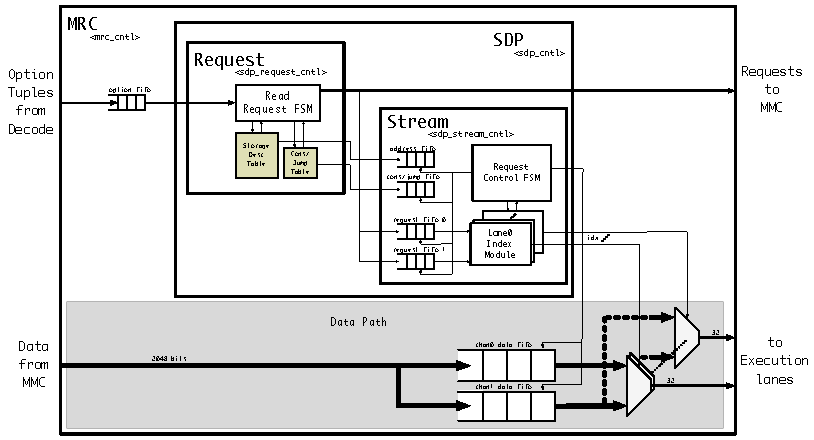
\includegraphics[width=1\linewidth]{mrcBlockDiagram}}
}
\center\caption{MRC block diagram}
\label{fig:MRC block diagram}
\end{figure}

The \ac{mrc} is one of the most complicated blocks in the system, it is also the largest but mainly because of the size of the data path \acp{fifo}.
There are two \ac{mrc} blocks instantiated in the manager, one for stream 0 and one for stream 1 in the execution lanes.

The \ac{mrc} uses the storage descriptor to identify the start address of the data and how the address should be incremented.
The \ac{sdp} block contains a request block and a stream block.
The request block uses the storage descriptor pointer to index into a small memory containing the actual storage descriptor. 
As described in section \ref{sec:Storage Descriptor}, the storage descriptor itself contains a start address and a pointer to a table containing consequtive and jump fields.
The starting address and consequtive/jump fields allow the request generator to make disjoint memory requests based on the \ac{roi} of the data. 
If the \ac{roi} is contiguous in memory, then there is one consequitive field and no jump field.

The request block generates memory requests based on the storage descriptor contents and number of lanes and sends the requests to the \ac{mmc}.
The request information is also sent to the stream block.
As the request block processes the storage descriptor start address and consequtive/jump fields it also send the information to the stream block.

The stream block is responsible for taking the 2048-bit memory data from the \ac{mmc} and directing words to each execution lane.
As the data is returned from the \ac{mmc}, it is placed in a channel 0 \ac{fifo} and a channel 1 \ac{fifo}. 
The stream block has a per execution lane index module each of which generates an index to the channel and word.
The index is used to multiplex the data to the execution lane stream.
The per execution lane index module is required to account for bank and page boundaries in the \ac{roi} as described in sections \ref{sec:AccessingANStates} and \ref{sec:Storage Descriptor}.
The lane index module uses the storage descritpor information to generate a memory location address which includes channel, bank, page and word addresses.
The location address is them matched to the request at the head of the two request \acp{fifo}, and it a match occurs, the data is passed to the execution lane bus.
If there is no match, the index module requests the request and data \acp{fifo} are read. The request control \ac{fsm} will ony read the \ac{fifo} if all lane index modules make a read request.
This is done because as data is stored in memory, if the data crosses a bank, page or cacheline boundary the execution lanes must be allowed to get out of sync.


\subsection{\Acf{rdp}}
\label{sec:RDP}
The \ac{rdp} is responsible for taking the result data from the \ac{pe} and determining which \ac{ssc} it should be stored (see figure \ref{fig:RDP block diagram}).

\begin{figure}[h]
\centering
\captionsetup{justification=centering}
\captionsetup{width=.9\linewidth}
\centerline{
\mbox{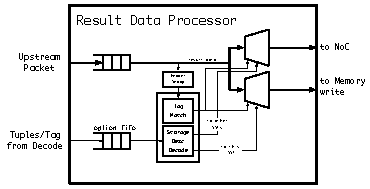
\includegraphics[width=0.85\linewidth]{rdpBlockDiagram}}
}
\center\caption{Result data processor}
\label{fig:RDP block diagram}
\end{figure}

The \ac{rdp} receives a descriptor from the decoder which includes storage descriptor information and the tag associated with an operation sent to the \ac{pe}.
The information is stored in a \ac{fifo} and as data is returned to the manager over the upstream stack bus, the \ac{rdp} matches the return data tag with the head of the \ac{fifo}.
Currently the return data is in order but to support an expansive architecture the tag is provided to and checked by the \ac{rdp}.

When the data is matched to the tag, the \ac{rdp} examines all the storage descriptor pointers. The pointers include \ac{ssc} index in the \acp{msb} and the \ac{rdp} constructs an \ac{ssc} bit-field.
Once the descriptors have been parsed, if one of the destinations is the local \ac{ssc} \ac{dram}, the \ac{rdp} passed the descriptor and data to the system conntroller which in turn passes it to the \ac{mwc}.
If the destination(s) include other \acp{ssc}, the \ac{rdp} provides the \ac{ssc} bitfield along with the data to the \ac{noc}.


\subsection{\Acf{mwc}}
\label{sec:MWC}

The \acf{mwc} receives data from two sources, the \ac{noc} via the system conntroller and the \ac{rdp}.
The \ac{mwc} uses the storage descriptor provided with the data to identify the write address.
The \ac{mwc} does not store the data immediately, it places the data in a small crude cache which has enough storage for two pages per channel.
A block diagram of the \ac{mwc} can be seen in figure \ref{fig:MWC block diagram}.
\begin{figure}[h]
\centering
\captionsetup{justification=centering}
\captionsetup{width=.9\linewidth}
\centerline{
\mbox{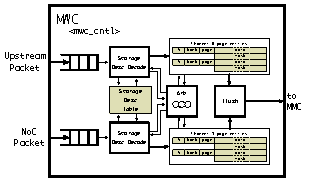
\includegraphics[width=0.85\linewidth]{mwcBlockDiagram}}
}
\center\caption{MWC block diagram}
\label{fig:MWC block diagram}
\end{figure}
As data is received from the \ac{rdp} or \ac{noc}, the addresses are compared to the cache entry and if page address match occurs and the corresponding word is invalid, the data is stored in the cache.
If a page miss occurs, the contents of one of the entries is written to memory and the new data stored in the cache.

This crude cache was provided for two reasons, first even though write efficiency was not anticipated to be an issue, as described in section \ref{sec:writingANStates}, it was anticipated that the addresses from multiple operations may occur in consequive address and by coalescing data would make writes more efficient.
The more important reason was to provide expansibility and by accounting for a small cache future work, such as host data downloads would have less of an impact on logic area.


\section{Processing Engine}
\label{sec:pe}

A block diagram of the \ac{pe} can be seen in figure \ref{fig:PE block diagram}.
\begin{figure}[h]
\centering
\captionsetup{justification=centering}
\captionsetup{width=.9\linewidth}
\centerline{
\mbox{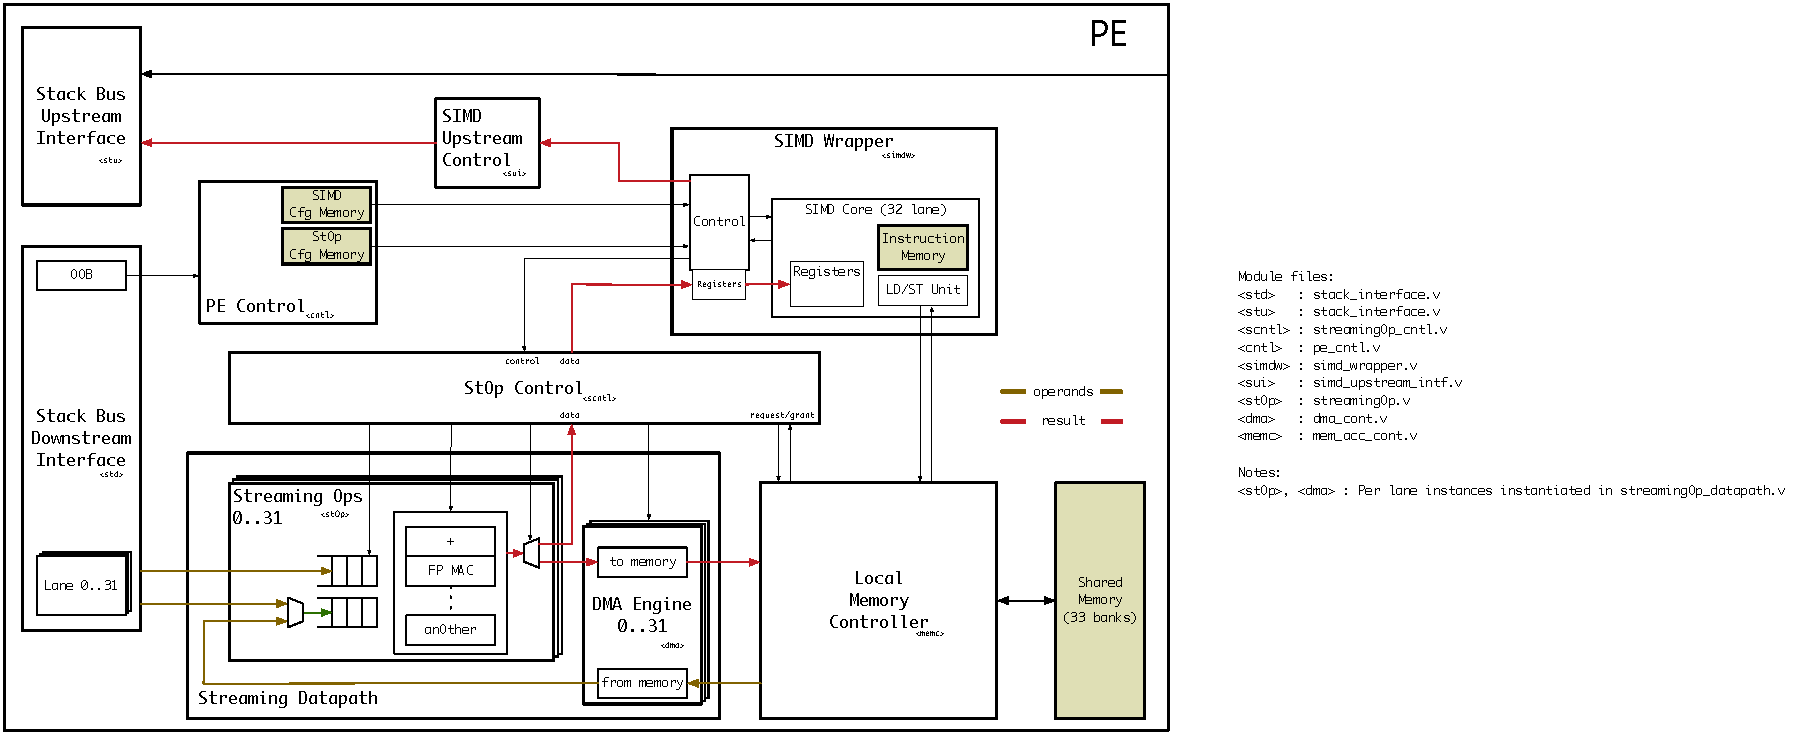
\includegraphics[width=1\linewidth]{PE}}
}
\center\caption{PE block diagram}
\label{fig:PE block diagram}
\end{figure}

\subsection{Configuration}
\label{sec:peConfiguration}

The manager sends configuration information to the \ac{pe} over the downstream \ac{oob} bus.
The \ac{oob} packet contains option tuples used by the \ac{pe} controller to configure functions within the \ac{pe}.
The controller extracts the \ac{stop} and \ac{simd} operation pointers from the appropriate option tuple value.
The \ac{stop} pointer is used to point to a local \ac{stop} configuration which contains the various configuration data required by the \ac{stop} function.
The configuration data includes:
\begin{outline}
    \1 \ac{stop} operation type
    \1 Number of active execution lanes
    \1 Source of the argument data, which can be downstream data from the manager or from the small local \ac{sram}
    \1 Destination of the result data, which can be the \ac{simd} and/or the small local \ac{sram}
\end{outline}
Once the information is provided to the \ac{stop} block and the pointer provided to the \ac{simd}, the operation is immediately started.
Currently only \ac{stop} and \ac{simd} pointer option tuples are used.
An example of the downstream \ac{oob} transactions can be seen in figure \ref{fig:Downstream OOB transactions}. This example shows both normal and extended option tuples.

\begin{figure}[h]
  % the [] contains position info e.g. [!t] means here
  \centering
  \captionsetup{justification=centering}

  \begin{minipage}{1\textwidth}
    \centering
    \captionsetup{justification=centering, skip=10pt}
    \begin{minipage}[t]{1\textwidth}
      \begin{minipage}[t]{1\textwidth}
        \begin{center}
          \begin{bytefield}[bitwidth=0.49em, endianness=big]{38}
            \bitheader{0, 31, 37} \\
            \bitbox{2}{\rotatebox{90}{\tiny SOM}} & \bitbox{4}{\tiny type} & \colorbitbox{optiontype!40}{8}{\tiny option \\ \vspace{-0em}type} & \colorbitbox{optionvalue!40}{8}{\tiny option \\ \vspace{-0em}value} & \colorbitbox{optiontype!40}{8}{\tiny option \\ \vspace{-0em}type} & \colorbitbox{optionvalue!40}{8}{\tiny option \\ \vspace{-0em}value}   \\
            \bitbox{2}{\rotatebox{90}{\tiny MOM}} & \bitbox{4}{\tiny type} & \colorbitbox{optiontype!40}{8}{\tiny extd option \\ \vspace{-0em}type} & \colorbitbox{optionvalue!40}{24}{\tiny option \\ \vspace{-0em}value} \\
            \bitbox[]{38}{$\vdots$} \\[1ex]                                                                                                                                                                          
            \bitbox{2}{\rotatebox{90}{\tiny EOM}} & \bitbox{4}{\tiny type} & \colorbitbox{optiontype!40}{8}{\tiny option \\ \vspace{-0em}type} & \colorbitbox{optionvalue!40}{8}{\tiny option \\ \vspace{-0em}value} & \colorbitbox{optiontype!40}{8}{\tiny option \\ \vspace{-0em}type} & \colorbitbox{optionvalue!40}{8}{\tiny option \\ \vspace{-0em}value}   \\
          \end{bytefield}
        \end{center}
      \end{minipage}
  \end{minipage}
  \begin{minipage}{1\textwidth}
      \centering
      \begin{minipage}[t]{0.28\textwidth}
        \vspace{1mm}
        \centering
        \begin{adjustbox}{width=1\textwidth}
            \footnotesize
            \begin{tabular}{ |c|c|  }
              \hline
              \rowcolor{gray!50}
              \multicolumn{2}{|c|}{Type} \\
              \hline
              \rowcolor{gray!25}
              type[3:0] & Description  \\
              \hline
              2     & Operation configuration \\
              other & NA \\
              \hline
            \end{tabular}
        \end{adjustbox}
      \end{minipage}
      \vspace{-2mm}
      \center\caption{Downstream OOB data transactions}
      \label{fig:Downstream OOB transactions}
    \end{minipage}
    \begin{minipage}[t]{1\textwidth}
      \vspace{7mm}
      \centering
      %\begin{adjustbox}{width=1\textwidth}
        \centering
        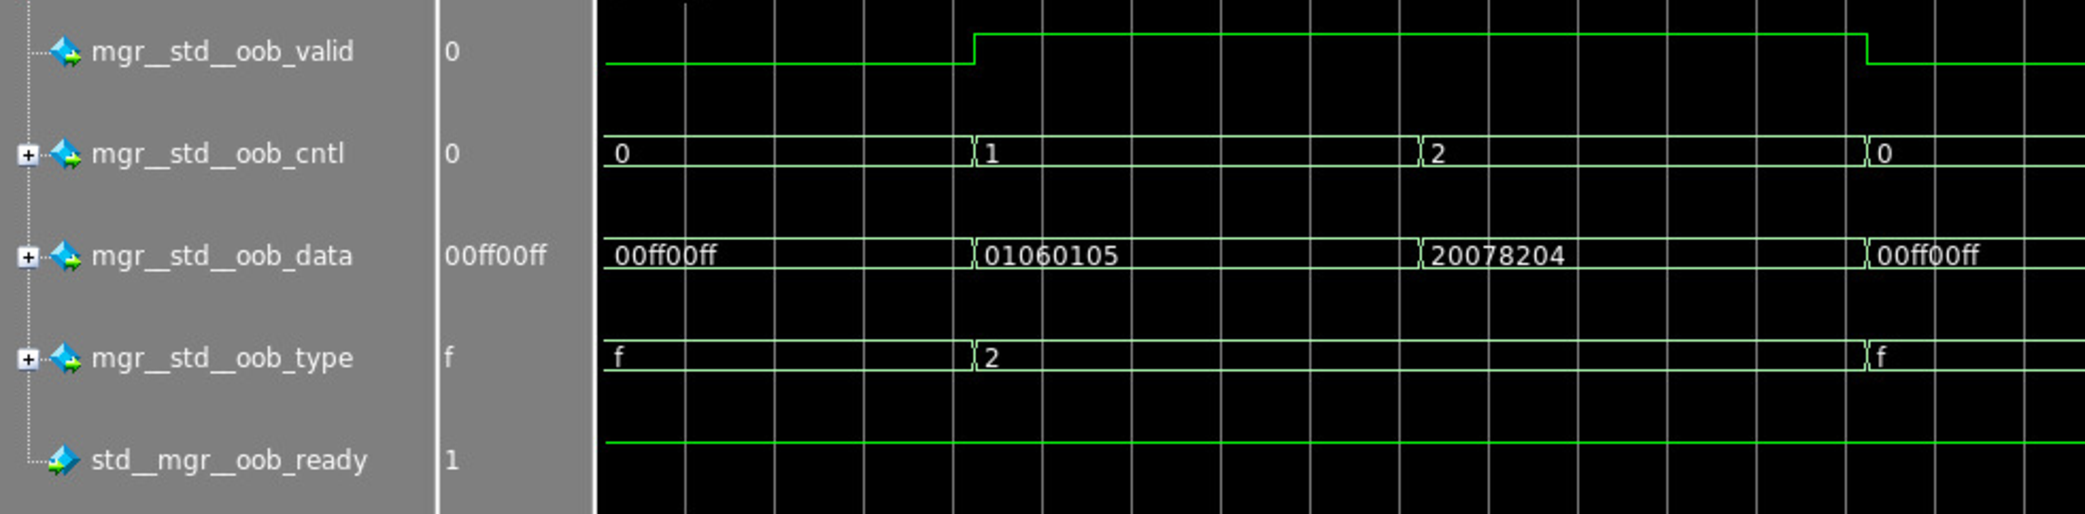
\includegraphics[scale=0.35]{stack_down_oob_waveform}
      %\end{adjustbox}
      \captionsetup{justification=centering, skip=10pt}
      \captionof{figure}{Downstream OOB simulation waveform}
      \label{fig:Downstream OOB simulation waveform}
    \end{minipage}
  \end{minipage}
\end{figure}


\subsection{PE Controller}
\label{sec:PE Cntl}

The \ac{pe} controller takes \ac{oob} control packets stored in an nterface \ac{fifo} and extracts the \ac{stop} and \ac{simd} pointers.
The \ac{stop} pointer is used to index into a small \ac{sram} which contains the long instruction word used to select the \ac{stop} functio and where to place the result.
The \ac{simd} pointer is passed to the \ac{simd} wrapper along with the tag associated with the operation.
When the \ac{stop} has completed the operation, the \ac{pe} controller takes the next operation from the \ac{oob} \ac{fifo}.
The \ac{simd} wrapper contains an interface \ac{fifo} and the \ac{pe} controller will only pause if the \ac{simd} wrapper interface asserts flow control.
A block diagram of the \ac{pe} controller can be seen in figure \ref{fig:PE Controller block diagram}}.
\begin{figure}[h]
% the [] contains position info e.g. [!H] means here
% H 	Place exactly at spot in source text
% h 	Place approximately at spot in source test
% t 	Place at top of page
% b 	Place at bottom of page
% p 	Place on page for floats only
% ! 	Override internal LaTeX parameters for determining float position
\centering
\captionsetup{justification=centering}
\captionsetup{width=0.9\textwidth}
\centerline{
\mbox{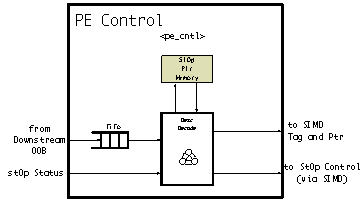
\includegraphics[angle=0, width=0.75\textwidth]{PEcntlBlockDiagram}}
}
\center\caption{PE controller block diagram}
\label{fig:PE Controller block diagram}
\end{figure}


\subsection{Streaming Operations}
\label{sec:stOps}

There is a \ac{stop} module for each execution lane and the \acp{stop} are designed to operate on data passed from the manager at or near line-rate. 
If line-rate cannot be maintained, an interface \ac{fifo} flow-control mechanism is employed to slow the data from the manager.
Once the \ac{stop} has processed the data, it passes the result to the \ac{simd}. Note in some cases the result can be placed in local \ac{sram} or sent to both \ac{sram} and \ac{simd}.

It should also be stated that while the \ac{stop} is processing the current data, the \ac{simd} may be operating on the result of the previous operation. 
It is expected the \ac{simd} will have completed the previous operation before the \ac{stop} completes the current operation, but again, if necessary a flow control mechanism between \ac{simd} and \ac{stop} will be engaged if the \ac{simd} is not ready.

There is provision for one of the inputs into the \ac{stop} module to be from the local memory via a local \ac{dma} controller. Although this is designed and tested, this processing path is for future work.
A block diagram of the \ac{stop} can be seen in figure \ref{fig:stOp block diagram}}.
\begin{figure}[h]
\centering
\captionsetup{justification=centering}
\captionsetup{width=0.9\textwidth}
\centerline{
\mbox{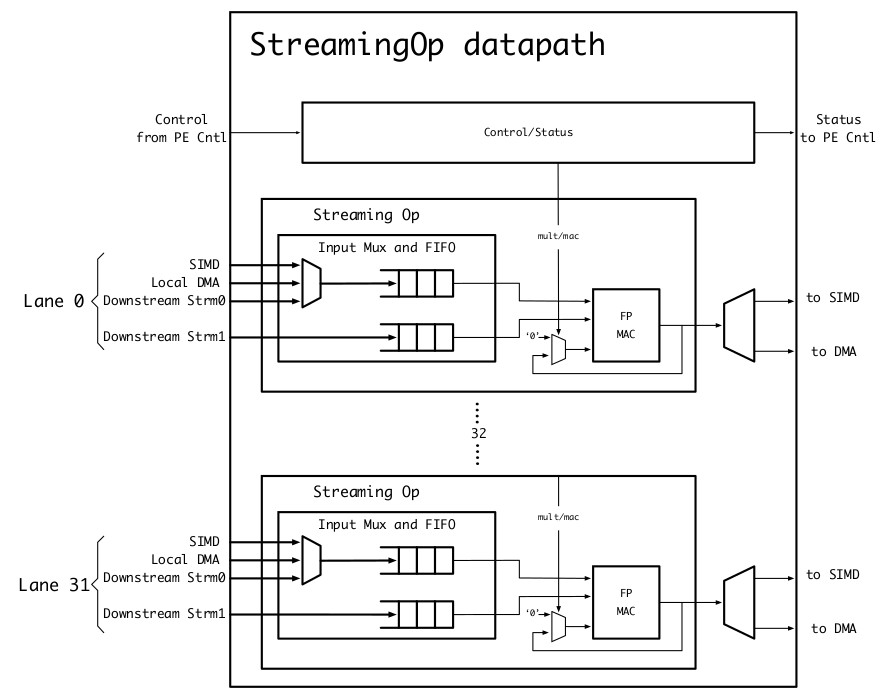
\includegraphics[angle=0, width=.75\textwidth]{streamingOpBlockDiagram}}
}
\center\caption{Streaming operations block diagram}
\label{fig:stOp block diagram}
\end{figure}


\subsection{SIMD}
\label{sec:simd}

The \ac{simd} takes the operation from the \ac{pe} controller and indexes into a small memory. This memory contains a \ac{pc} for the \ac{simd} along with control information for processing the \ac{stop} result inside the wrapper.
This work does not put a high level of importance on the \ac{simd} as the functionality provided by the \ac{simd} is to provide a level of flexibility for future work.
Therefore an actual \ac{simd} was not simulated and the data from the \ac{stop} was processed by logic in the \ac{simd} wrapper block, as can be seen in figure \ref{fig:simd wrapper block diagram}.
However, it was important to include the \ac{simd} in the area portion of the study.
To account for the \ac{simd}, a dummy \ac{simd} instance was instantiated inside the \ac{simd} wrapper and in the area layout study a placement blockage was used based 32 lane, 32-bit \ac{simd} from \cite{schabel2014diss}.
In practice, the \ac{simd} will take the result data from the \ac{stop} and perform the operation starting at the \ac{pc} indicated by the \ac{simd} operation pointer provided by the \ac{pe} controller.
The \ac{simd} performs the specified operation on the data provided by the \ac{stop} which can be passed directly to the \ac{simd} or provided indirectly in \ac{simd} local memory.
In most cases, the \ac{simd} operation \ac{an} activation function which in the baseline system is the \ac{relu} function.
When the \ac{simd} wrapper has completed its operation, it passes the result to the upstream controller to be returned to the manager.
\begin{figure}[h]
\centering
\captionsetup{justification=centering}
\captionsetup{width=0.9\textwidth}
\centerline{
\mbox{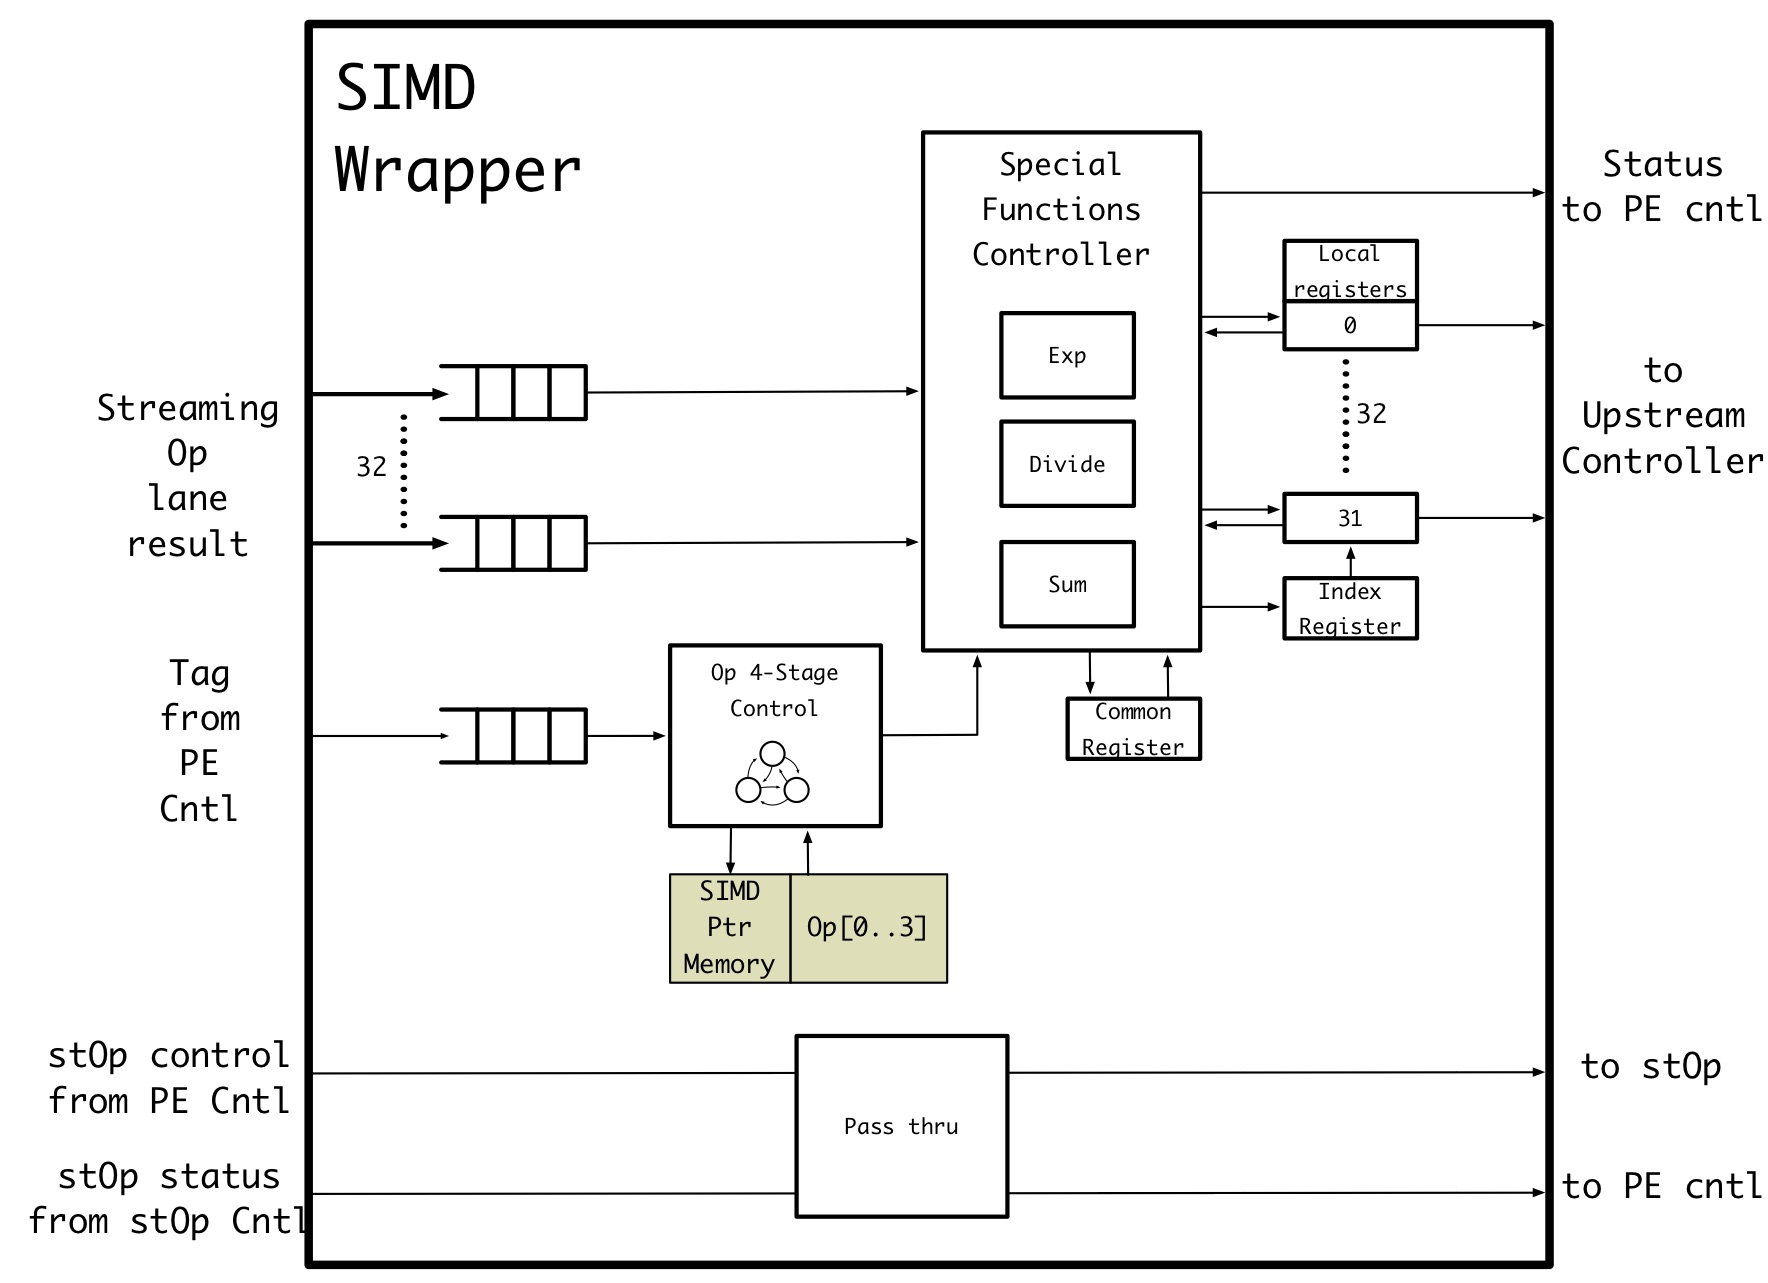
\includegraphics[angle=0, width=.75\textwidth]{SIMDwrapperBlockDiagram}}
}
\center\caption{SIMD wrapper block diagram}
\label{fig:simd wrapper block diagram}
\end{figure}


\subsection{DMA Controller and Local memory}
\label{sec:Dma Cntl}

The \ac{pe} provides some local \ac{sram} for future use.
Both the \ac{stop} and the \ac{simd} will have access to the local memory.
In the case of the \ac{stop}, one of the \ac{stop} inputs can be sourced from the local memory using a \ac{dma} comtroller.
The \ac{dma} controller is controlled from fields in the instruction word in the \ac{pe} controller.
The paths from the local memory to the \ac{stop} and from the \ac{stop} to the local memory have been tested.


\subsection{Upstream controller}
\label{sec:Upstream controller}}

The upstream controller takes the data from the \ac{simd} and a tag from the \ac{pe} controller and sends it to the manager.
The format of the upstream transactions can be seen in figure \ref{fig:Upstream data transactions}.
The upstream packet format accomodates both data and tag to be transmitted or just the tag.
The upstream format allows sending tag only is to accomodate a sync flush operation without data being returned to the manager.
Currently only the tag and data mode has been implemented.

\begin{figure}[h]
  % the [] contains position info e.g. [!t] means here
  \centering
  \captionsetup{justification=centering}

  \begin{minipage}{1\textwidth}
    \centering
    \captionsetup{justification=centering, skip=10pt}
    \begin{minipage}[t]{0.45\textwidth}
      \begin{flushright}
        \begin{bytefield}[bitwidth=0.49em, endianness=big]{22}
          \bitheader{0, 16, 21} \\
          \bitbox{2}{\rotatebox{90}{\tiny SOM}} & \bitbox{2}{\rotatebox{90}{\tiny type}} & \bitbox{2}{\tiny PV} & \bitbox{16}{\tiny OOB Data} \\
          \bitbox[]{22}{$\vdots$} \\[1ex]                                      
          \bitbox{2}{\rotatebox{90}{\tiny EOM}} & \bitbox{2}{\rotatebox{90}{\tiny type}} & \bitbox{2}{\tiny PV} & \bitbox{16}{\tiny OOB Data} 
        \end{bytefield}
      \end{flushright}
    \end{minipage}
    \begin{minipage}[t]{0.45\textwidth}
      \begin{flushleft}
        \hspace{1mm}
        \begin{bytefield}[bitwidth=0.1em, endianness=big]{128}
          \bitheader{0,127} \\
          \begin{rightwordgroup}{\scriptsize $1$st Cycle}
            \bitbox{32}{\tiny Data} 
            \bitbox{32}{\tiny Data} 
            \bitbox{32}{\tiny Data} 
            \bitbox{32}{\tiny Data} 
          \end{rightwordgroup}  \\
          \bitbox[]{128}{$\vdots$} \\[1ex]
          \begin{rightwordgroup}{\scriptsize $n$th Cycle}
            \bitbox{32}{\tiny Data} 
            \bitbox{32}{\tiny Data} 
            \bitbox{32}{\tiny Data} 
            \bitbox{32}{\tiny Data}
          \end{rightwordgroup} 
        \end{bytefield}
      \end{flushleft}
    \end{minipage}
  \end{minipage}
  \begin{minipage}{1\textwidth}
    \centering
    \begin{minipage}[t]{0.25\textwidth}
      \vspace{3mm}
      \centering
      \begin{adjustbox}{width=1\textwidth}
          \footnotesize
          \begin{tabular}{ |c|c|  }
            \hline
            \rowcolor{gray!50}
            \multicolumn{2}{|c|}{Type} \\
            \hline
            \rowcolor{gray!25}
            type[1:0] & Description  \\
            \hline
            0     & OOB=Tag, Data valid \\
            1     & OOB=NA, Data valid \\
            2     & OOB=Tag, Data invalid \\
            3     & NA \\
            \hline
          \end{tabular}
      \end{adjustbox}
    \end{minipage}
    \begin{minipage}[t]{0.2\textwidth}
      \vspace{3mm}
      \centering
      \begin{adjustbox}{width=1\textwidth}
          \footnotesize
          \begin{tabular}{ |c|c|  }
            \hline
            \rowcolor{gray!50}
            \multicolumn{2}{|c|}{ Number of valid words} \\
            \hline
            \rowcolor{gray!25}
            PV[1:0] & Description  \\
            \hline
            0     & One word valid \\
            1     & Two words valid \\
            2     & Three words valid \\
            3     & Four words valid \\
            \hline
          \end{tabular}
      \end{adjustbox}
    \end{minipage}
  \end{minipage}
  \vspace{-3mm}
  \center\caption{Upstream data transactions}
  \label{fig:Upstream data transactions}
\end{figure}



\begin{sidewaysfigure}[h]
% the [] contains position info e.g. [!H] means here
% H 	Place exactly at spot in source text
% h 	Place approximately at spot in source test
% t 	Place at top of page
% b 	Place at bottom of page
% p 	Place on page for floats only
% ! 	Override internal LaTeX parameters for determining float position
\centering
\captionsetup{justification=centering}
\captionsetup{width=0.9\textwidth}
\centerline{
\mbox{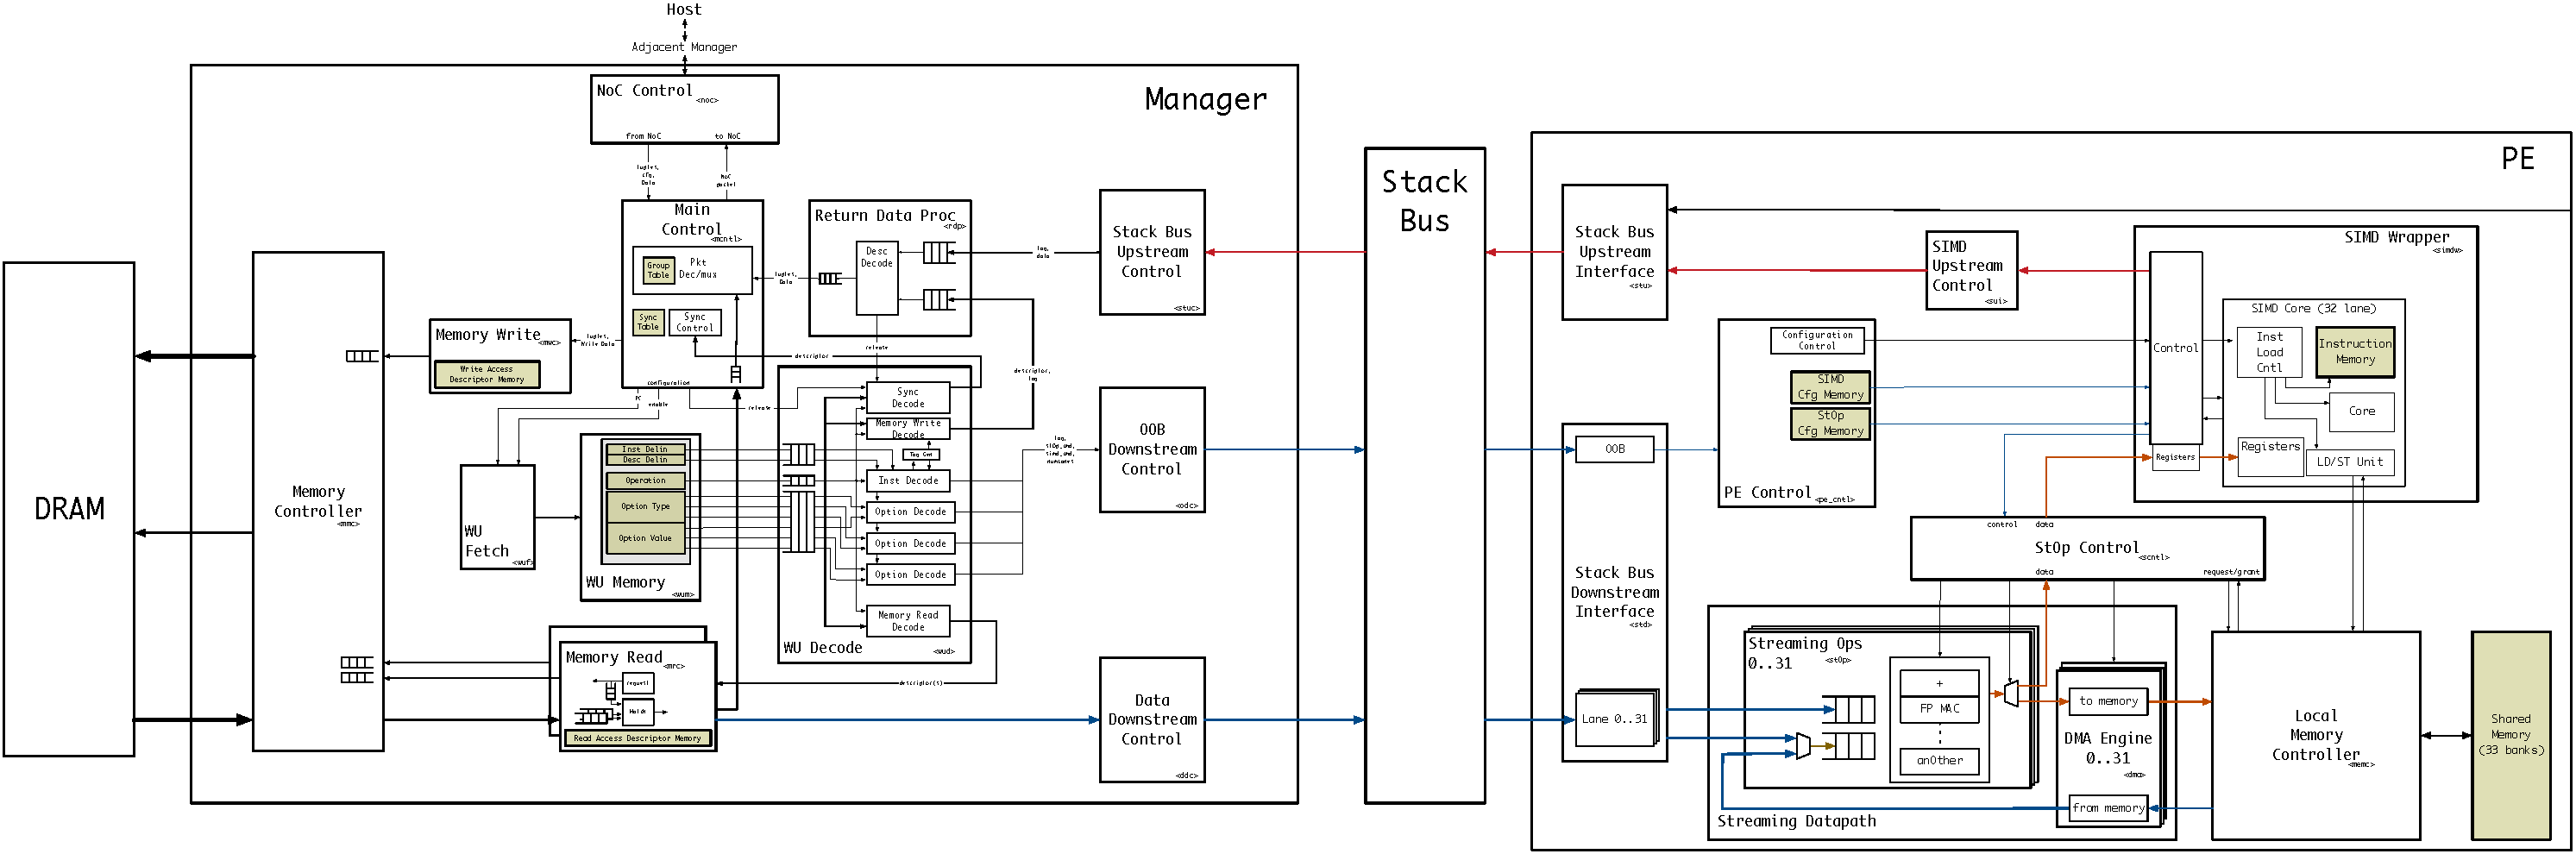
\includegraphics[angle=0, width=1.0\textwidth]{DetailedBlockDiagram}}
}
\center\caption{Sub-System Column (SSC) Block Diagram}
\label{fig:DetailedBlockDiagram}
\end{sidewaysfigure}


